\documentclass[a4paper,12pt]{article}

\usepackage[serbian]{babel}
\usepackage[T2A]{fontenc} 
\usepackage[utf8]{inputenc} 
\usepackage[margin=1in]{geometry}
\usepackage{csquotes}
\usepackage[nottoc]{tocbibind}
\usepackage[backend=biber]{biblatex}
\usepackage{authblk}
\usepackage{tikz}
\usepackage{subfigure}
\usepackage{algorithm2e}
\usepackage{graphicx}

\RestyleAlgo{ruled}

\addbibresource{sample.bib}

\title{Algoritham brišuće prave za određivanje hijerarhije između kružnica}
\author{Andrija Urošević\\\textit{Univerzitet u Beogradu, Matematički fakultet}\\\textit{Katedra za računarstvo i informatiku}\\\texttt{andrija.urosevic@matf.bg.ac.rs}}
\date{Avgust, 2023.}

\begin{document}

\maketitle\

Opis algoritma i implementacionih detalja algoritma brišuće prave za određivanje hijerarhije između kružnica. Algoritam je zasnovan i implementiran po uzoru na rad: \emph{Deok-Soo Kim, Byunghoon Lee, Kokichi Sugihara: A Sweep-Line Algorithm for the Inclusion Hierarchy among Circles} \cite{kls06}.

\section{Opis problema}

Neka je dat skup kružnica $\mathcal{C} = \{C_1, C_2, \ldots, C_n\}$, gde je kružnica $C_i$ definisana sa centrom $(x_i, y_i)$ i poluprečnikom $r_i$. Pretpostavimo da kružnice mogu da sadrže druge kružnice dok presek između dve kružne linije nije dozvoljen. Za dati skup $\mathcal{C}$, želimo da konstrušemo hijerarhiju između kružnica, tj.\ da odredimo relaciju sadržanja između svake dve kružnice iz $\mathcal{C}$. 

Jedan primer kružnica i odgovarajuće hijerarhije između kružnica je dat na slici~\ref{fig:example}.

\begin{figure}
\begin{center}
    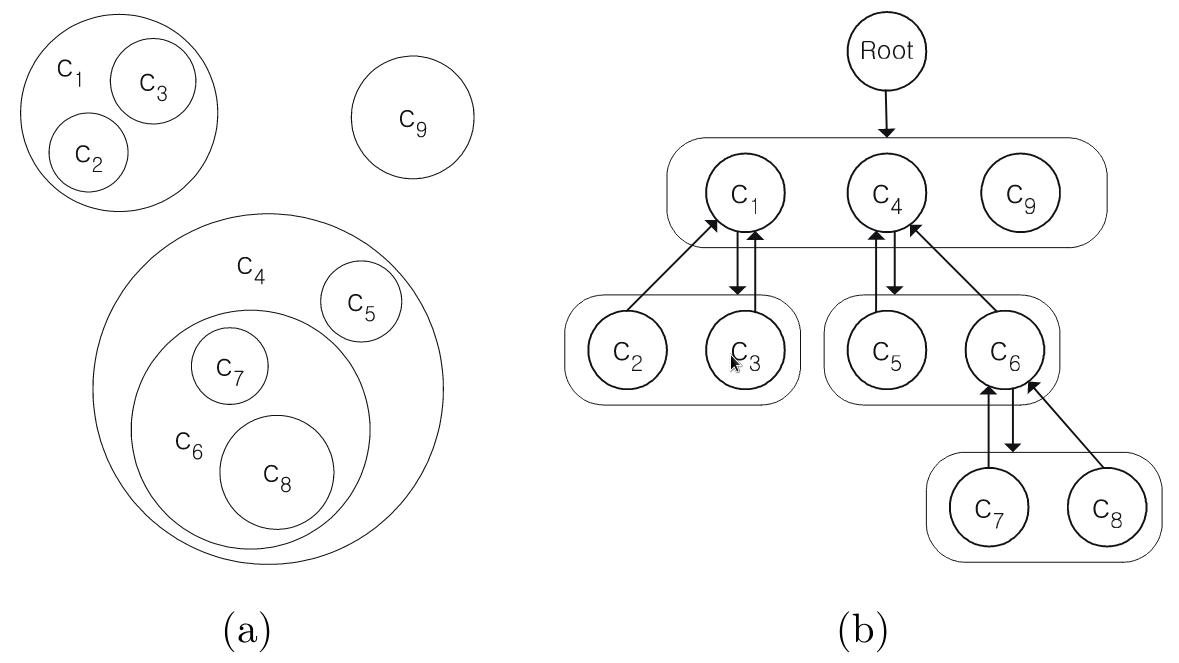
\includegraphics[width=0.8\textwidth]{imgs/inc.png}
\end{center}
    \caption{Primer kružnica: (a) Grafički prikaz kružnica; (b) Hijerarhija između kružnica.}
\label{fig:example}
\end{figure}


\section{Algoritam}

Razmotrićemo prvo naivni algoritam grube sile, koji radi u $O(n^2)$ vremenu. Nako toga primetićemo da je algoritam moguće rešiti mnogo efikasnije u $O(n \log n)$ vremenu, ako koristimo tehniku brišuće prave zajedno sa odgovarajućim strukturama podataka.

\subsection{Algoritam grube sile}
\label{sub:brute}

Ideja algoritma grube sile je u proveri svih parova različitih kružnica da li se jedna sadrži u drugoj. Provera da li je neka kružnica sadržana u drugoj kružnici se složenosti $O(1)$, pa je ukupna složenost algoritma $O(n^2)$.

Algoritam grube sile je opisan algoritmom~\ref{alg:brute}.

\begin{algorithm}
    \caption{Gruba sila}\label{alg:brute}
    \KwData{Skup kružnica $\mathcal{C} = \{C_1, C_2, \ldots, C_n\}$}
    \For{$C_i \in \mathcal{C}$}{%
        \For{$C_j \in \mathcal{C}$} {%
            \If{$i \neq j$ i $C_i$ sadrži $C_j$} {%
                $C_i.sadrzi \gets C_j$;
            }
        }
    }
\end{algorithm}

\subsection{Algoritam brišuće prave}
\label{sub:sweep}

Metod brišuće prave se oslanja na vertikalnu liniju, \emph{brišuću pravu}, koja prolazi sa leva na desno. Na tom putu ona česno ne menja zadate osobine, ali postoje tačke u kojima dolazi do promene zadatih osobina i te tačke se nazivaju \emph{tačke događaja}.

\subsubsection{Događaji}
\label{subsub:event}

Neka su najlevlja i najdešnja ekstremna tačka kružnice $C_i$ obeležene sa $L_i$ i $R_i$, respektivno. Zaključujemo da ih ima $2n$ za $n$ kružnica. Ekstremne tačke sortirane po $x$ koordinatama čine listu događaja. Ekstremne tačke koje odgovaraju najlevljim ekstremnim tačkama kružnica su događaji \emph{rađanja}, dok su ekstremne tačke koje odgovaraju najdešnjim tačkama kružnica događaju \emph{umiranja}. Slika~\ref{fig:event} ilustruje primer tri kružnice i njihovu odgovarajuću listu događaja.

\begin{figure}
\begin{center}
    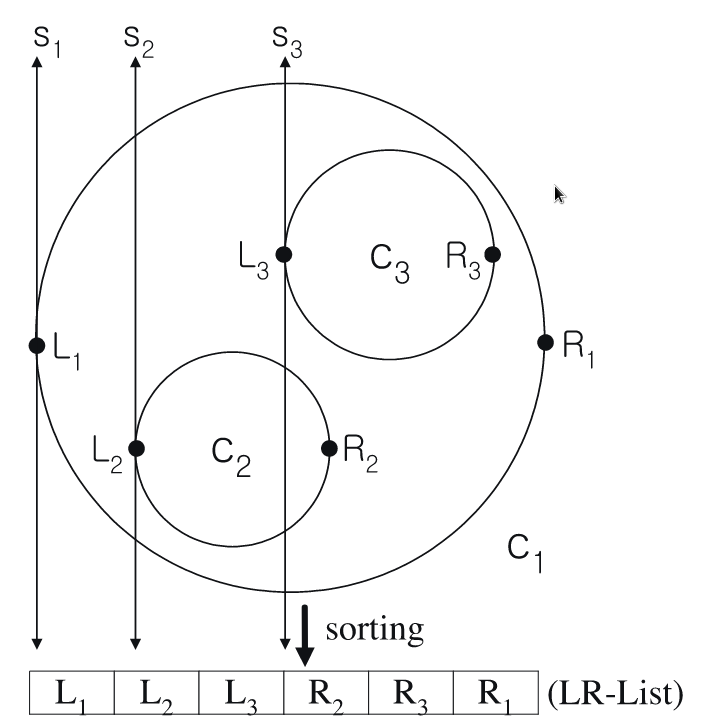
\includegraphics[width=0.5\textwidth]{imgs/event.png}
\end{center}
    \caption{Lista događaja}
\label{fig:event}
\end{figure}

\subsubsection{Generisanje intervala}
\label{subsub:intgen}

Brušuća prava je u svakom trenutku podeljena na \emph{intervale}. Granice intervala su presečne tačke obima kružnica i brišuće prave. Čuvaju se u crveno crnim stablima kako bi obezbedili efikasnu pretragu, umetanje i brisanje u $O(\log n)$ vremenu.

Svaki interval $i$ sadrži dve vrednosti za donju i gornju granicu. Ako se granice intervale poklope takav interval nazivamo \emph{nula interval}. Slika~\ref{fig:open} predstavlja 4 scenarija brišuće prave i intervale u njima.

Inicijalno u $S_0$ imamo samo jedan interval $i_1$. U trenutku $L_1$, interval $i_1$ se deli tri intervala $[i_i, i_2, i_3]$. U trenutku $L_2$, interval $i_2$ se deli na $[i_2, i_4, i_5]$, te lista intervala postaje $[i_1, i_2, i_4, i_5, i_3]$. Pored toga, u trenutku $L_2$, kako je interval $i_2$ unutar kružnice $C_1$ možemo zaključiti da je kružnica $C_2$ sadržana u kružnici $C_1$. 

Opštije, ako se tačka $L_j$, nalazi unutar interval $i_k$, onda interval $i_k$ delima na tri intervala $[i_k, i_{m+1}, i_{m+2}]$, gde je $m$ trenutan ukupan broj intrvala. Pri tome, ako je kružnica $C_k$ unutar intervala $i_k$, a $C_j$ kružnica kojoj odgovara najlevija ekstremna tačka $L_j$, onda $C_k$ sadrži $C_j$.

\begin{figure}
\begin{center}
    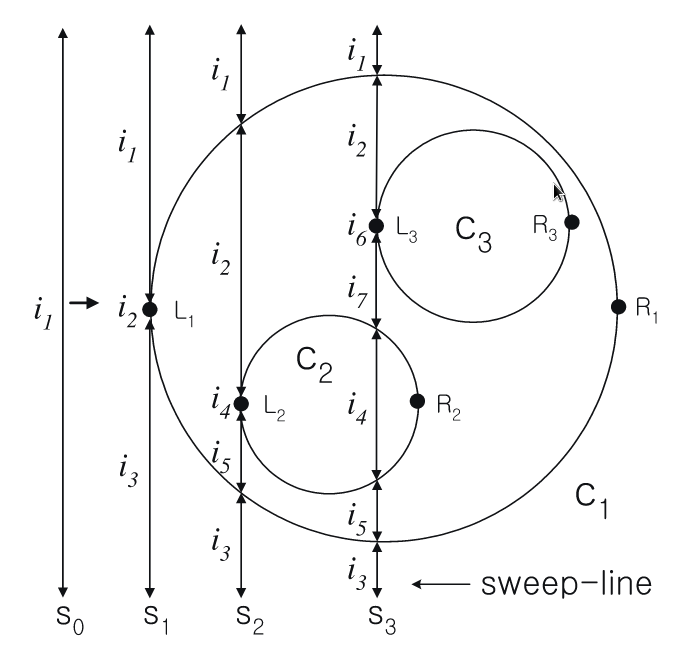
\includegraphics[width=0.5\textwidth]{imgs/open.png}
\end{center}
    \caption{Nastajanje novih itervala na događajima rađanja.}
\label{fig:open}
\end{figure}

\subsubsection{Brisanje intervala}
\label{subsub:intdel}

Kada naiđemo na najdešnju ekstremu tačku, tj.\ događaj umiranja, treba ažurirati intervale. Na slici~\ref{fig:close} je prikazana detekcija događaja umiranja, zajedno sa brisanjem dva intervala koja su nastala pri rađanju odgovarajuće kružnice.

\begin{figure}
\begin{center}
    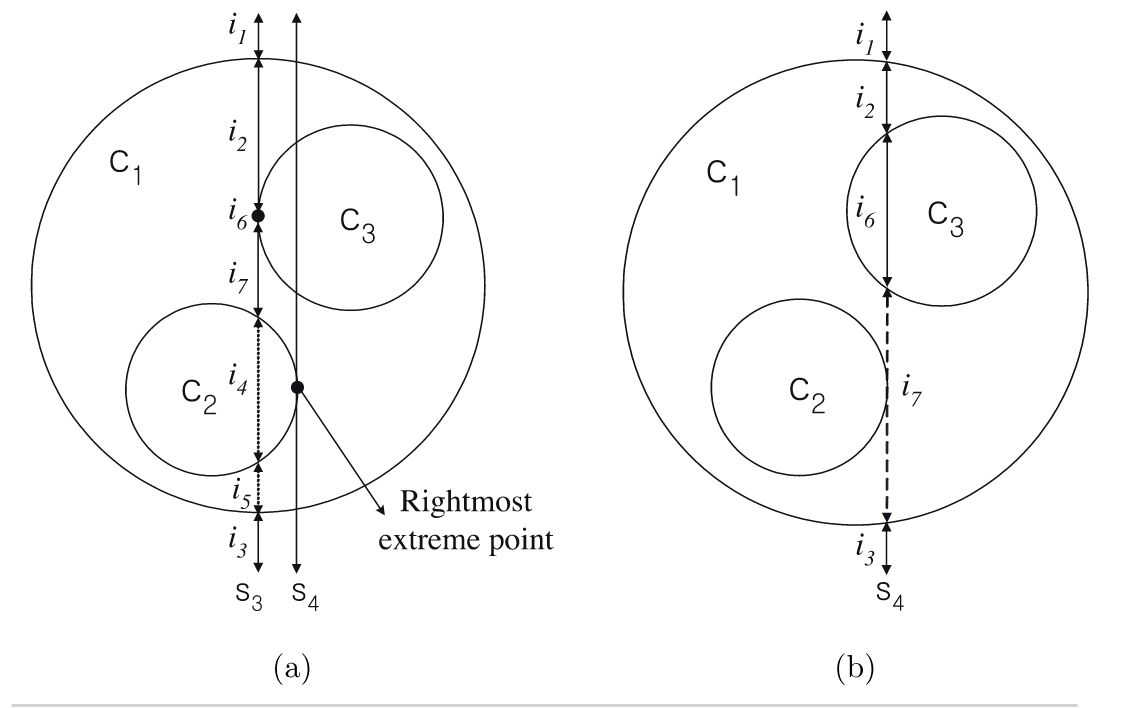
\includegraphics[width=0.7\textwidth]{imgs/close.png}
\end{center}
    \caption{Brisanje dva intervala na događaju umiranja: (a) $i_4$ i $i_5$ su odgovarajući intervali za brisanje; (b) modifikovani intervali brišuće prave nako brisanja dva intervala.}
\label{fig:close}
\end{figure}

\subsubsection{Algoritam}
\label{subsub:sweep}

Algoritma brišuće prave za detekciju hijerarhije između kružnica je prikazan algoritmom~\ref{alg:sweep}.

\begin{algorithm}
    \caption{Brušuća prava}\label{alg:sweep}
    \KwData{Skup kružnica $\mathcal{C} = \{C_1, C_2, \ldots, C_n\}$}
    Inicijalizuje praznu listu događaja $E$\;
    \For{$C_i \in \mathcal{C}$}{%
        $E \gets E + \{Event(C_i, open)\}$\;
        $E \gets E + \{Event(C_i, close)\}$\;
    }
    Sortiraj ekstremne tačke $E$ u neopadajućem poretku po njihovim $x$ koordinatama\;
    Inicijalizuje crveno crno stablo intervala $I \gets \{i_0\}$, gde je $i_0 = (-\infty, +\infty)$\;
    \For{$e_j \in E$}{%
        \eIf{$e_j.open$}{%
            $i = (y, y') \gets I.find(e_j.y)$\;
            \If{$i_2$ sadrži $C_k$}{%
                $C_k.sadrzi \gets e_j.circle$\;
            }
            $i' \gets (y, e_j.y)$\;
            $i'' \gets (e_j.y, y')$\;
            $I \gets I + \{i', i''\}$\;
        }{%
            $i' \gets I.find(e_j)$\;
            $i \gets i'.prev$\;
            $i'' \gets i'.next$\;
            $I \gets I - \{i', i''\}$\;
        }
    }
\end{algorithm}

\section{Strukture podataka}
\label{sec:data}

\paragraph{Kružnica}
\label{par:circ}
Svaka kužnica ima pridruženi centar (par realnih brojeva) i poluprečnik (neki realan broj). Pored toga svaka od njih ima definisanu funkciju za pronalaženje gornje i donje tačke sa obima za zadatu $x$ koordinatu. Ova funkcija je od značaja u pronalaženju odgovarajućeg intervala u crveno crnom stablu intervala.

\paragraph{Događaj}
\label{par:event}
Događaj je predstavljen odgovarajućom $x$ koordinatom, indikatorom da li je događaj rađenje/umiranje kuržnice, i pokazivačom na odgovarajuću kružnicu.

\paragraph{Interval}
\label{par:Interval}
Interval je ključna struktura koja treba da definiše između ostalog i poredak u crveno crnom stablu. Od veliko značaja je ažurirati ovu strukturu korektno tokom izvođenja algoritma kako bi se očuvao poredak. Struktura čuva pokazivač na kružnicu koju sadrži, pored toga, čuva i gornju i donju granicu preko pokazivača na gornju i donju kružnicu. Kako brišuća prava preseca obim kružnice u potencijalno dve tačke treba voditi računa o tome da li uzimamo gornju ili donju tačku za svaku od graničnih kružnica.

Na osnovu toga možemo lako izračunati gornju i donju granicu intervala. Kako intervala nemaju presek lako je definisati poredak između njih:
\[i_1 < i_2 \iff i_1.LB + \epsilon < i_2.LB \lor i_1.UB + \epsilon < i_2.UB.\]
Jednakost između dva intervala se sada lako definiše kao 
\[i_1 = i_2 \iff \neg (i_1 < i_2) \land \neg (i_2 < i_1).\]

\subsection{Crveno crna stabla}
\label{sub:rbt}

Za čuvanje intervala koristimo crveno crno stablo. 

\paragraph{Pretraga intervala}
\label{par:ints}

Svaki put kada bršuća prava naiđe na novu kružnicu generiše se najlevlja ekstremna tačka. Treba odrediti u kom se intervalu ona nalazi. Kako se intervali čuvaju u crveno crnom stablu odgovarajući interval se može pronaći u $O(\log n)$ vremnu. Tokom pretrage treba korisiti nove granice intervala koje računamo za trenutnu $x$ vrednost brišuće prave. 

Primetimo da ovo neće promeniti poredak intervala.

\paragraph{Insertovanje intervala}
\label{par:inti}

Kada naiđemo na najlevlju ekstremu taču kružnice dva nova intervala se kreiraju. Njihovo dodavanje u crveno crno stablo zahteva $O(\log n)$ vremena.

\paragraph{Brisanje intervala}
\label{par:intd}

Kada nastane događaj umiranja na najdešnjoj ekstemnoj tački kuržnice treba obrisati odgovarajuće intervale iz crveno crnog stabla. Dva intervala brišemo, dok treći ažuriramo tako da njegovo sledeće računanje gornje i donje granice ostane konzistentno.
Ove operacije se mogu izvršiti u $О(\log n)$ vremenu.

\section{Složenost algoritma}
\label{sec:complexity}

Generisanje liste događaja i njeno sortiranje zahteva $O(n \log n)$ koraka, kako se za svaku kružnicu generišu dva događaja, događaj rađanja i događaj umiranja, za levu i desnu ekstremnu tačku kružnice, respektivno. Inicijalizacija crveno crnog stabla interval ima konstantnu složenost. Za svaku događaj u najgorem slučaju vršimo $O(\log n)$ operacija, te obrada svih događaja ima složenost $O(n \log n)$.

Ukupa složenost algoritma je $O(n \log n)$.

\printbibliography[title={Literatura}]

\end{document}
